% !TEX root = Anforderungsliste.tex
\begin{center}
\begin{tabular}{|p{1cm}|p{0.5cm}|p{5cm}|p{5cm}|p{1.5cm}|}\hline
 \textbf{4} & & \textbf{Fahrbahn} & & \\\hline
 4.1 & F & Maximale Fugenbreite zwischen den Spanplatten & <2mm & Alle\\\hline
 4.2 & F & Maximaler Überstand zwischen den Spanplatten & <2mm & Alle\\ \hline
 4.3 & F & Minimaler Abstand zu Hindernissen über der Fahrbahn &  $\geq$ 1m & Alle\\\hline
 4.4 & F & Minimaler Abstand zu Hindernissen um die Fahrbahn &  $\geq$ 50cm & Alle\\\hline
 4.5 & F & Die Farbe der abzufahrenden Spur ist grau und wird mit einer weissen gestrichelten Linie von der Gegenfahrbahn getrennt &   & Alle\\ \hline
 4.6 & F & Die Breite der weissen Mittellinien & 1cm $\pm$ 0.2 cm & Alle\\ \hline
 4.7 & F & Die Breite der Fahrstreifen & je 20cm $\pm$ 1cm & Alle\\ \hline
 4.8 & F & Begrenzungen der rechten Fahrspur (wann welcher Punkt zutrifft der Abbildung 1 entnehmen) & \begin{itemize} \item Durch die Trottoirkante gegeben (sofern ein Trottoir vorhanden ist)\item Mit einer weissen Linie markiert \item Nicht gekennzeichnet \end{itemize}  & Alle\\ \hline
 4.9 & F & Die Breite der weissen Linie an der rechten Fahrspur &  1cm $\pm$ 0.2cm & Alle\\ \hline
 4.10 & F & Der Abstand der weissen Linie an der rechten Fahrspur zur Mittellinie(jeweils von der Mitte der beiden Linien)&  20cm $\pm$ 1cm & Alle\\ \hline
 4.11 & F & Minimale Kurvenradius der Strassenmittellinie &  60cm $\pm$ 5cm & Alle\\ \hline
 4.12 & F & Die Breite des Trottoirs &  9cm $\pm$ 1cm & Alle\\ \hline
 4.13 & F & Die Höhe der Trottoirkante &  0.5cm $\pm$ 0.1cm & Alle\\ \hline
 4.14 & F & Das Trottoir ist fest und darf belastet werden & & Alle\\ \hline
 4.15 & F & Der Abstand von den auf dem Trottoir platzierten Objekten (z.B Bauarbeiter, Schranken, etc.) zu den Containern & $\geq$ 10cm & Alle\\ \hline
 4.16 & F & Die Länge des Start- und Zielparkfeld & 50cm $\pm$ 2cm & Alle\\ \hline
 4.17 & F & Die Breite des Start- und Zielparkfeld & 20cm $\pm$ 1cm & Alle\\ \hline
 4.18 & F & Drei Seiten der Start - und Zielfelder werden mit einer weissen Linie markiert. & & Alle\\ \hline
 4.19 & F & Die Breite der Randlinien der Felder & 1cm $\pm$ 0.2cm & Alle\\ \hline
 4.20 & F & Die vom Fahrzeug aus gesehene linke Randlinie im Startfeld ist wie die Mittellinie gekennzeichnet & & Alle\\\hline
 \end{tabular}
 \newpage
\begin{tabular}{|p{1cm}|p{0.5cm}|p{5cm}|p{5cm}|p{1.5cm}|}\hline
 4.21 & F & Es dürfen keine Gegenstände auf der Fahrbahn liegen oder auf die Fahrbahn ragen & & Alle\\\hline
 4.22 & F & Fahrbahn muss trocken sein & & Alle \\\hline
\end{tabular}\\[0.3cm]
\begin{tabular}{|p{1cm}|p{0.5cm}|p{5cm}|p{5cm}|p{1.5cm}|}\hline
 \textbf{5} & & \textbf{Äussere Einflüsse} & & \\\hline
 5.1 & F & Beleuchtung & Scheinwerfer Beleuchtung (analog PREN2 2015) & Alle\\\hline
 5.2 & F & Beleuchtung & Blinklichter sind nicht zugelassen & Alle\\\hline
 5.3 & F & Temperatur & 15-35 °C & Alle \\\hline
 \end{tabular}\\[0.3cm]
 \begin{tabular}{|p{1cm}|p{0.5cm}|p{5cm}|p{5cm}|p{1.5cm}|}\hline
 \textbf{6} & & \textbf{Sonstiges} & & \\\hline
 6.1 & F & Vorbereitungszeit von freigegebener Strecke bis Start Wettbewerb & 2 min & Alle \\\hline
 6.2 & F & Zeitaufwand für das Projekt & 6 ETCS x 30h x 7 Studenten = 1260h für PREN1 / für PREN2 analoge Anzahl an Stunden & Alle \\\hline
 6.3 & F & Budget & Gesammt: 500 CHF / für PREN1 max. 200 CHF & Alle \\\hline
 \end{tabular}\\[0.3cm]
 \textbf{Nicht beschriebene Punkte gemäss Aufgabenstellung und FAQ.}
\end{center}

\begin{figure}[ht]
	\centering									
	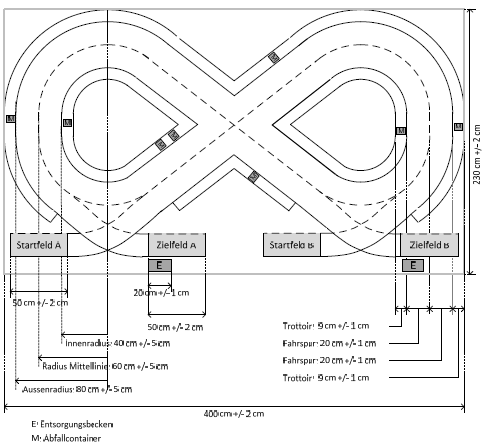
\includegraphics{Images/Fahrbahn.png}
	\caption{Die Fahrbahn mit den Bemessungen aus der Aufgabenstellung (nicht maßstäblich.)}
	\label{fig1}
	%Quelle: Aufgabenstellung_PREN1_H15_V2.pdf
\end{figure}